\documentclass[]{article}
\usepackage[left=1in,top=1in,right=1in,bottom=1in]{geometry}


%%%% more monte %%%%
% thispagestyle{empty}
% https://stackoverflow.com/questions/2166557/how-to-hide-the-page-number-in-latex-on-first-page-of-a-chapter
\usepackage{color}
% \usepackage[table]{xcolor} % are they using color?

% \definecolor{WSU.crimson}{HTML}{981e32}
% \definecolor{WSU.gray}{HTML}{5e6a71}

% \definecolor{shadecolor}{RGB}{248,248,248}
\definecolor{WSU.crimson}{RGB}{152,30,50} % use http://colors.mshaffer.com to convert from 981e32
\definecolor{WSU.gray}{RGB}{94,106,113}

%%%%%%%%%%%%%%%%%%%%%%%%%%%%

\newcommand*{\authorfont}{\fontfamily{phv}\selectfont}
\usepackage{lmodern}


  \usepackage[T1]{fontenc}
  \usepackage[utf8]{inputenc}




\usepackage{abstract}
\renewcommand{\abstractname}{}    % clear the title
\renewcommand{\absnamepos}{empty} % originally center

\renewenvironment{abstract}
 {{%
    \setlength{\leftmargin}{0mm}
    \setlength{\rightmargin}{\leftmargin}%
  }%
  \relax}
 {\endlist}

\makeatletter
\def\@maketitle{%
  \pagestyle{empty}
  \newpage
%  \null
%  \vskip 2em%
%  \begin{center}%
  \let \footnote \thanks
    {\fontsize{18}{20}\selectfont\raggedright  \setlength{\parindent}{0pt} \@title \par}%
}
%\fi
\makeatother






\usepackage{color}
\usepackage{fancyvrb}
\newcommand{\VerbBar}{|}
\newcommand{\VERB}{\Verb[commandchars=\\\{\}]}
\DefineVerbatimEnvironment{Highlighting}{Verbatim}{commandchars=\\\{\}}
% Add ',fontsize=\small' for more characters per line
\usepackage{framed}
\definecolor{shadecolor}{RGB}{248,248,248}
\newenvironment{Shaded}{\begin{snugshade}}{\end{snugshade}}
\newcommand{\AlertTok}[1]{\textcolor[rgb]{0.94,0.16,0.16}{#1}}
\newcommand{\AnnotationTok}[1]{\textcolor[rgb]{0.56,0.35,0.01}{\textbf{\textit{#1}}}}
\newcommand{\AttributeTok}[1]{\textcolor[rgb]{0.77,0.63,0.00}{#1}}
\newcommand{\BaseNTok}[1]{\textcolor[rgb]{0.00,0.00,0.81}{#1}}
\newcommand{\BuiltInTok}[1]{#1}
\newcommand{\CharTok}[1]{\textcolor[rgb]{0.31,0.60,0.02}{#1}}
\newcommand{\CommentTok}[1]{\textcolor[rgb]{0.56,0.35,0.01}{\textit{#1}}}
\newcommand{\CommentVarTok}[1]{\textcolor[rgb]{0.56,0.35,0.01}{\textbf{\textit{#1}}}}
\newcommand{\ConstantTok}[1]{\textcolor[rgb]{0.00,0.00,0.00}{#1}}
\newcommand{\ControlFlowTok}[1]{\textcolor[rgb]{0.13,0.29,0.53}{\textbf{#1}}}
\newcommand{\DataTypeTok}[1]{\textcolor[rgb]{0.13,0.29,0.53}{#1}}
\newcommand{\DecValTok}[1]{\textcolor[rgb]{0.00,0.00,0.81}{#1}}
\newcommand{\DocumentationTok}[1]{\textcolor[rgb]{0.56,0.35,0.01}{\textbf{\textit{#1}}}}
\newcommand{\ErrorTok}[1]{\textcolor[rgb]{0.64,0.00,0.00}{\textbf{#1}}}
\newcommand{\ExtensionTok}[1]{#1}
\newcommand{\FloatTok}[1]{\textcolor[rgb]{0.00,0.00,0.81}{#1}}
\newcommand{\FunctionTok}[1]{\textcolor[rgb]{0.00,0.00,0.00}{#1}}
\newcommand{\ImportTok}[1]{#1}
\newcommand{\InformationTok}[1]{\textcolor[rgb]{0.56,0.35,0.01}{\textbf{\textit{#1}}}}
\newcommand{\KeywordTok}[1]{\textcolor[rgb]{0.13,0.29,0.53}{\textbf{#1}}}
\newcommand{\NormalTok}[1]{#1}
\newcommand{\OperatorTok}[1]{\textcolor[rgb]{0.81,0.36,0.00}{\textbf{#1}}}
\newcommand{\OtherTok}[1]{\textcolor[rgb]{0.56,0.35,0.01}{#1}}
\newcommand{\PreprocessorTok}[1]{\textcolor[rgb]{0.56,0.35,0.01}{\textit{#1}}}
\newcommand{\RegionMarkerTok}[1]{#1}
\newcommand{\SpecialCharTok}[1]{\textcolor[rgb]{0.00,0.00,0.00}{#1}}
\newcommand{\SpecialStringTok}[1]{\textcolor[rgb]{0.31,0.60,0.02}{#1}}
\newcommand{\StringTok}[1]{\textcolor[rgb]{0.31,0.60,0.02}{#1}}
\newcommand{\VariableTok}[1]{\textcolor[rgb]{0.00,0.00,0.00}{#1}}
\newcommand{\VerbatimStringTok}[1]{\textcolor[rgb]{0.31,0.60,0.02}{#1}}
\newcommand{\WarningTok}[1]{\textcolor[rgb]{0.56,0.35,0.01}{\textbf{\textit{#1}}}}



\title{\textbf{\textcolor{WSU.crimson}{The Ideal
Human}} \newline \textbf{\textcolor{WSU.gray}{How body proportions of
modern humans compare to those of Leonardo da Vinci's Vitruvian Man}}  }
 

%  

% \author{ \Large true \hfill \normalsize \emph{} }
\author{\Large Jailee
Foster\vspace{0.05in} \newline\normalsize\emph{Washington State
University}  }


\date{November 10, 2020}
\setcounter{secnumdepth}{3}

\usepackage{titlesec}
% See the link above: KOMA classes are not compatible with titlesec any more. Sorry.
% https://github.com/jbezos/titlesec/issues/11
\titleformat*{\section}{\bfseries}
\titleformat*{\subsection}{\bfseries\itshape}
\titleformat*{\subsubsection}{\itshape}
\titleformat*{\paragraph}{\itshape}
\titleformat*{\subparagraph}{\itshape}

% https://code.usgs.gov/usgs/norock/irvine_k/ip-092225/


%\titleformat*{\section}{\normalsize\bfseries}
%\titleformat*{\subsection}{\normalsize\itshape}
%\titleformat*{\subsubsection}{\normalsize\itshape}
%\titleformat*{\paragraph}{\normalsize\itshape}
%\titleformat*{\subparagraph}{\normalsize\itshape}

% https://tex.stackexchange.com/questions/233866/one-column-multicol-environment#233904
\usepackage{environ}
\NewEnviron{auxmulticols}[1]{%
  \ifnum#1<2\relax% Fewer than 2 columns
    %\vspace{-\baselineskip}% Possible vertical correction
    \BODY
  \else% More than 1 column
    \begin{multicols}{#1}
      \BODY
    \end{multicols}%
  \fi
}





\usepackage{natbib}
\setcitestyle{aysep={}} %% no year, comma just year
% \usepackage[numbers]{natbib}
\bibliographystyle{./../biblio/ormsv080.bst}



\usepackage[strings]{underscore} % protect underscores in most circumstances




\newtheorem{hypothesis}{Hypothesis}
\usepackage{setspace}


%%%%%%%%%%%%%%%%%%%%%%%%%%%%%%%%%%%%%%%%%%%%%%%%%%%%%
%%% MONTE ADDS %%%

\usepackage{fancyhdr} % fancy header 
\usepackage{lastpage} % last page 

\usepackage{multicol}


\usepackage{etoolbox}
\AtBeginEnvironment{quote}{\singlespacing\small}
% https://tex.stackexchange.com/questions/325695/how-to-style-blockquote


\usepackage{soul}			%% allows strike-through
\usepackage{url}			%% fixes underscores in urls
\usepackage{csquotes}		%% allows \textquote in references
\usepackage{rotating}		%% allows table and box rotation
\usepackage{caption}		%% customize caption information
\usepackage{booktabs}		%% enhance table/tabular environment
\usepackage{tabularx}		%% width attributes updates tabular
\usepackage{enumerate}		%% special item environment
\usepackage{enumitem}		%% special item environment

\usepackage{lineno}		%% allows linenumbers for editing using \linenumbers
\usepackage{hanging}


\usepackage{mathtools}  	%% also loads amsmath
\usepackage{bm}		%% bold-math
\usepackage{scalerel}	%% scale one element (make one beta bigger font)

\newcommand{\gFrac}[2]{ \genfrac{}{}{0pt}{1}{{#1}}{#2} }

\newcommand{\betaSH}[3]{  \gFrac{\text{\tiny #1}}{{\text{\tiny #2}}}\hat{\beta}_{\text{#3}}   }
\newcommand{\betaSB}[3]{              ^{\text{#1}} _{\text{#2}} \bm{\beta} _{\text{#3}}                   }  %% bold
\newcommand{\bigEQ}{  \scaleobj{1.5}{{\ }= } }
\newcommand{\bigP}[1]{  \scaleobj{1.5}{#1 } }





\usepackage{endnotes}  % he already does this ...
\renewcommand{\enotesize}{\normalsize}
% https://tex.stackexchange.com/questions/99984/endnotes-do-not-be-superscript-and-add-a-space
\renewcommand\makeenmark{\textsuperscript{[\theenmark]}} % in brackets %
% https://tex.stackexchange.com/questions/31574/how-to-control-the-indent-in-endnotes
\patchcmd{\enoteformat}{1.8em}{0pt}{}{}

\patchcmd{\theendnotes}
  {\makeatletter}
  {\makeatletter\renewcommand\makeenmark{\textbf{[\theenmark]} }}
  {}{}



% https://tex.stackexchange.com/questions/141906/configuring-footnote-position-and-spacing

\addtolength{\footnotesep}{5mm} % change to 1mm

\renewcommand{\thefootnote}{\textbf{\arabic{footnote}}}
\let\footnote=\endnote
%\renewcommand*{\theendnote}{\alph{endnote}}
%\renewcommand{\theendnote}{\textbf{\arabic{endnote}}}


\renewcommand*{\notesname}{ENDNOTES}

\makeatletter
\def\enoteheading{\section*{\notesname
  \@mkboth{\MakeUppercase{\notesname}}{\MakeUppercase{\notesname}}}%
  \mbox{}\par\vskip-2.3\baselineskip\noindent\rule{.5\textwidth}{0.4pt}\par\vskip\baselineskip}
\makeatother


\renewcommand*{\contentsname}{CONTENTS}

\renewcommand*{\refname}{Bibliography}


%\usepackage{subfigure}
\usepackage{subcaption}

\captionsetup{labelfont=bf}  % Make Table / Figure bold

%%% you could add elements here ... monte says .... %%%
%\usepackage{mypackageForCapitalH}


%%%%%%%%%%%%%%%%%%%%%%%%%%%%%%%%%%%%%%%%%%%%%%%%%%%%%

% set default figure placement to htbp
\makeatletter
\def\fps@figure{htbp}
\makeatother


% move the hyperref stuff down here, after header-includes, to allow for - \usepackage{hyperref}

\makeatletter
\@ifpackageloaded{hyperref}{}{%
\ifxetex
  \PassOptionsToPackage{hyphens}{url}\usepackage[setpagesize=false, % page size defined by xetex
              unicode=false, % unicode breaks when used with xetex
              xetex]{hyperref}
\else
  \PassOptionsToPackage{hyphens}{url}\usepackage[draft,unicode=true]{hyperref}
\fi
}

\@ifpackageloaded{color}{
    \PassOptionsToPackage{usenames,dvipsnames}{color}
}{%
    \usepackage[usenames,dvipsnames]{color}
}
\makeatother
\hypersetup{breaklinks=true,
            bookmarks=true,
            pdfauthor={Jailee Foster (Washington State University)},
             pdfkeywords = {},  
            pdftitle={The Ideal Human: How body proportions of modern
humans compare to those of Leonardo da Vinci's Vitruvian Man},
            colorlinks=true,
            citecolor=blue,
            urlcolor=blue,
            linkcolor=magenta,
            pdfborder={0 0 0}}
\urlstyle{same}  % don't use monospace font for urls

% Add an option for endnotes. -----

%
% add tightlist ----------
\providecommand{\tightlist}{%
\setlength{\itemsep}{0pt}\setlength{\parskip}{0pt}}

% add some other packages ----------

% \usepackage{multicol}
% This should regulate where figures float
% See: https://tex.stackexchange.com/questions/2275/keeping-tables-figures-close-to-where-they-are-mentioned
\usepackage[section]{placeins}



\pagestyle{fancy}   
\lhead{\textcolor{WSU.crimson}{\textbf{ The Ideal Human }}}
\chead{}
\rhead{\textcolor{WSU.gray}{\textbf{  Page\ \thepage\ of\ \protect\pageref{LastPage} }}}
\lfoot{}
\cfoot{}
\rfoot{}


\begin{document}
	
% \pagenumbering{arabic}% resets `page` counter to 1 
%    

% \maketitle

{% \usefont{T1}{pnc}{m}{n}
\setlength{\parindent}{0pt}
\thispagestyle{plain}
{\fontsize{18}{20}\selectfont\raggedright 
\maketitle  % title \par  

}

{
   \vskip 13.5pt\relax \normalsize\fontsize{11}{12} 
   
\textbf{\authorfont Jailee Foster} \hskip 15pt \emph{\small Washington
State University}   

}

}








\begin{abstract}

    \hbox{\vrule height .2pt width 39.14pc}

    \vskip 8.5pt % \small 

\noindent In this article, I compare three of the proportions found in
Leonardo da Vinci's Vitruvian Man to measurements collected on adults in
2020. This is achieved by first writing the height of each subject as a
factor of their head height, their foot length, and their hand length.


    



    
    \hbox{\vrule height .2pt width 39.14pc}
    \vskip 5pt 
    \hfill \textbf{\textcolor{WSU.gray}{ November 10, 2020 } }
    \vskip 5pt 
    
\end{abstract}


\vskip -8.5pt



 % removetitleabstract

\noindent  

\section{Introduction}
\label{sec:intro}

\paragraph{}

Over 500 years ago, Leonardo da Vinci crafted the \emph{Vitruvian Man},
a drawing depicting his idea of the ideal proportions a human body
should possess. Da Vinci's drawing was influenced by Roman architect
Vitruvius' \emph{De architectura}, a book detailing the design of the
human body \citep{Wikipedia:Vitruvian}.

\section{Research Question: How do the proportions in \emph{Vitruvian Man} compare to the measurements of adults today?}
\label{sec:rq}

\paragraph{}

I set out to compare three proportions described in
\emph{Vitruvian Man}, the proportion of height to each of hand length,
head height, and foot length. The sample consisted of 196 adults (over
18) from a range of ethnicities.

\subsection{Is the average humans height equal to ten times the length of their hand?}
\paragraph{}

Hand length is defined as the length from the tip of the middle finger
to the wrist when the hand is open. Text that is found on the drawing
itself can be translated as ``\ldots the length of the hand is one-tenth
of the height of a man'' \citep{Wikipedia:Vitruvian}. \label{sec:rq2}

\subsection{Is the average human's height equal to 8 times the height of their head?}
\label{sec:rq3}
\paragraph{}

Part of the text from the drawing is translated to ``from below the chin
to the top of the head is one-eighth of the height of a man''
\citep{Wikipedia:Vitruvian}. Therefore, I will explore whether or not it
is valid to assume that the average human's height is equal to the
height of 8 of their heads.

\subsection{Is the average human's height equal to 7 times the length of their foot?}
\label{sec:rq4}
\paragraph{}

The length of the foot can be found by measuring from the tip of the big
toe to the edge of the heel. Da Vinci noted in his drawing that ``the
foot is one-seventh of the height of a man''
\citep{Wikipedia:Vitruvian}.

\begin{figure}[!ht]
    \begin{subfigure}[h]{\textwidth}
    \centering
    %  trim={<left> <lower> <right> <upper>}
    % https://shantoroy.com/latex/add-subfig-in-latex/
            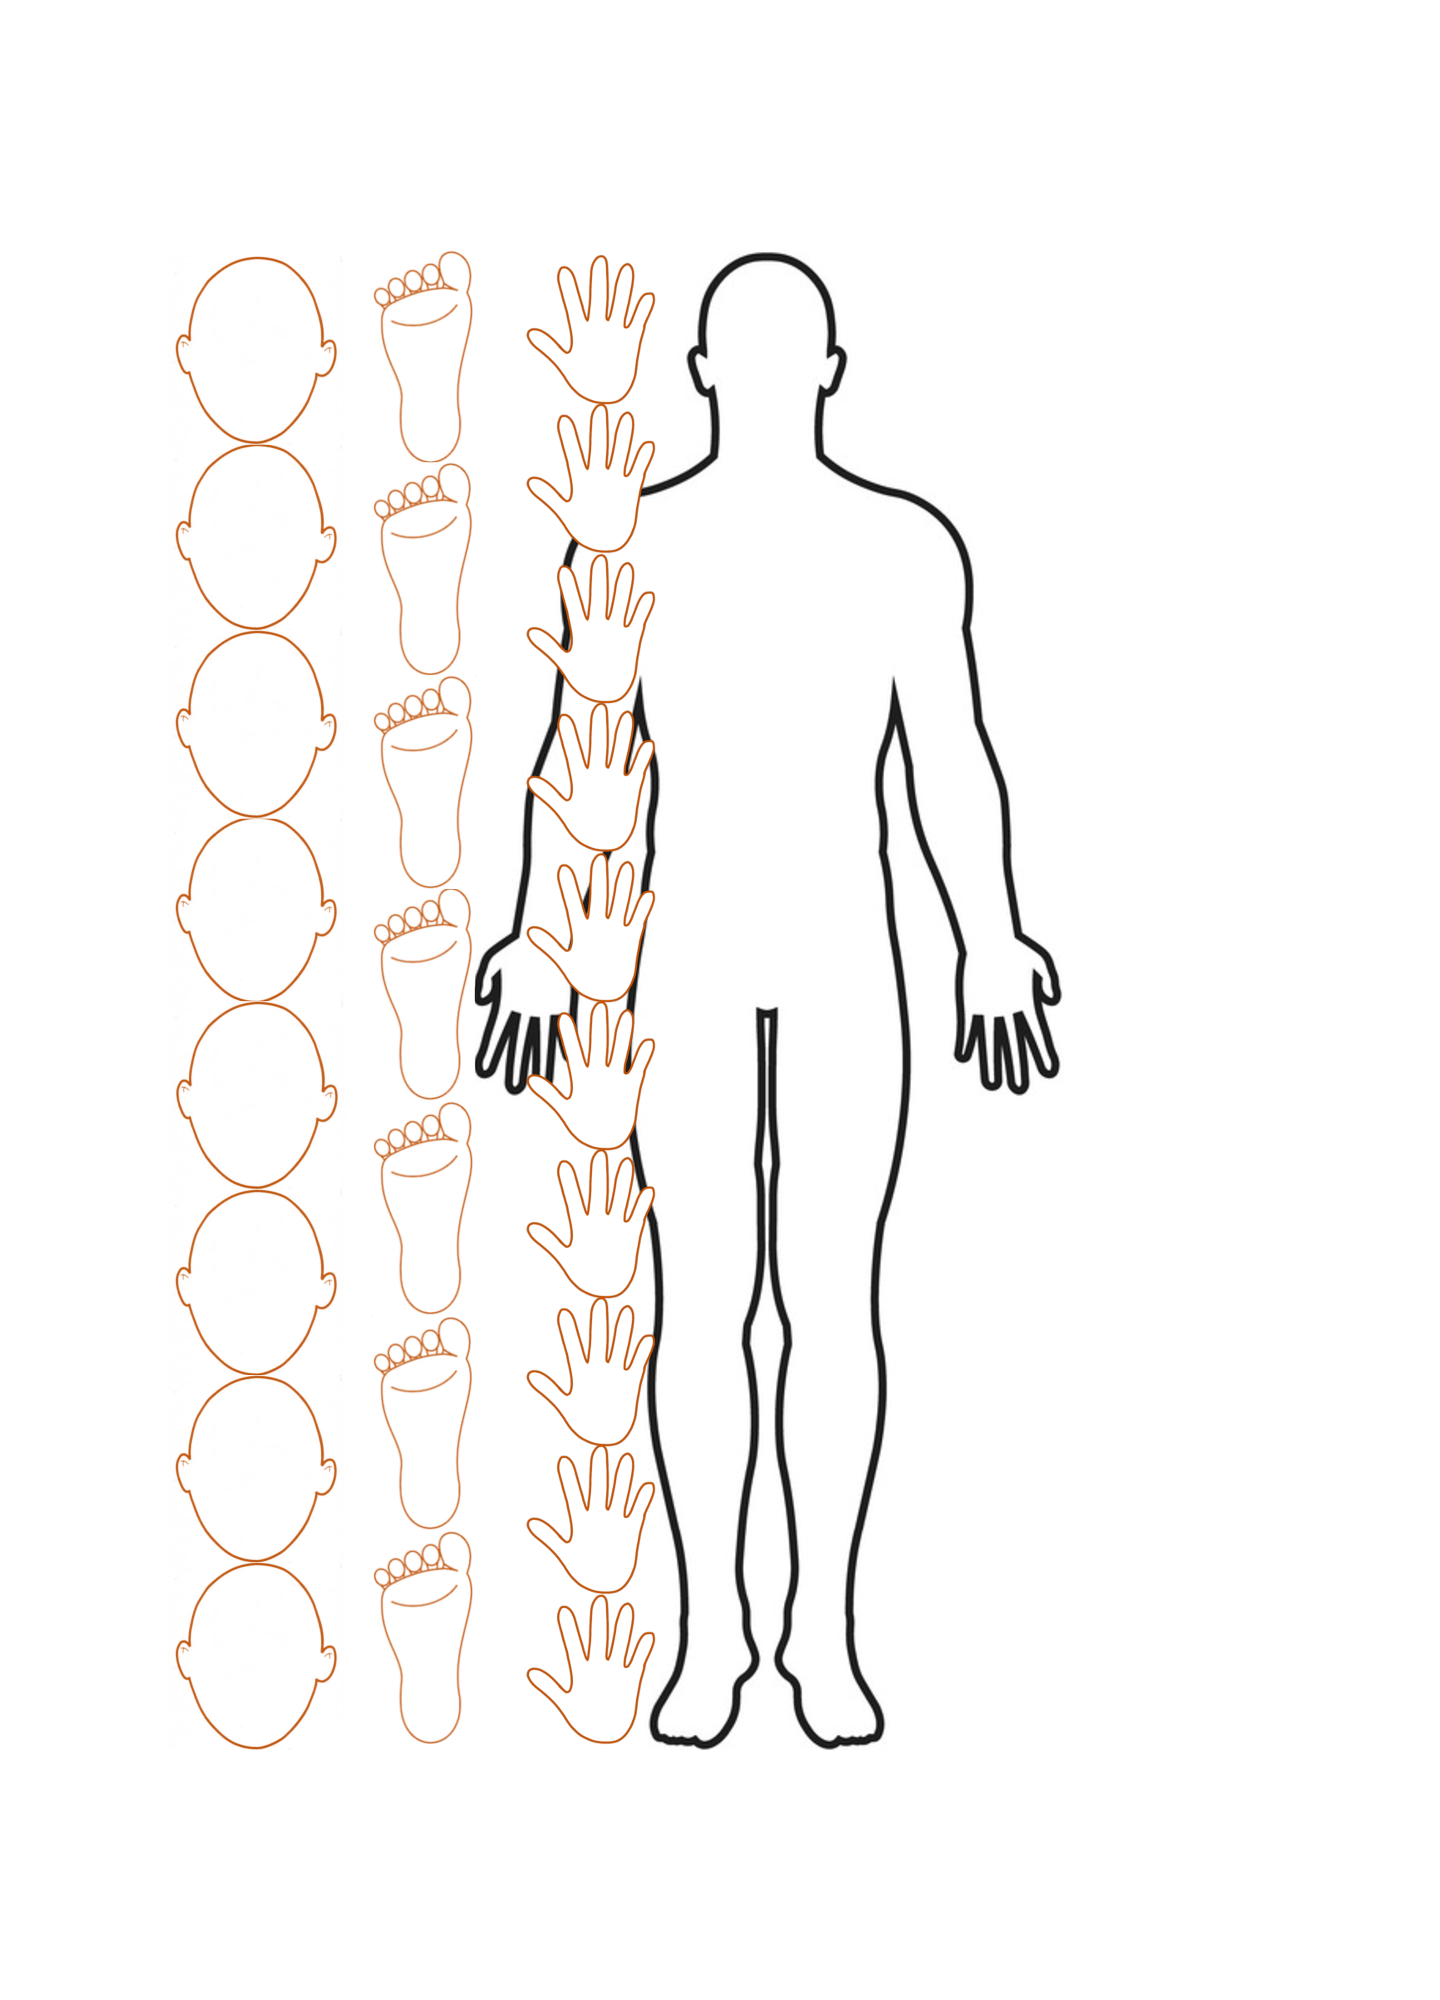
\includegraphics[trim = 0 0 0 0,clip,scale=0.5]{figures/final-image.pdf}
        \label{fig:sub-first}
    \end{subfigure}
    \vspace{2.5mm}
    \hrule
    \vspace{2.5mm}
        \caption{\textbf{Vitruvian Man proportions shown visually:} Are there differences in the ideal measurements as presented by Leonardo Da Vinci in his Vitruvian man and measurements performed on 196 adults? Specifically, is the height of an adult equivalent to 10 times his hand length, 8 times his head height, and 7 times his foot length? \citet{Wikipedia:Vitruvian} \tiny\emph{\newline\newline Figure components came from the following websites: \newline https://www.vectorstock.com/royalty-free-vector/illstration-human-body-icon-outline-vector-29311539\newline  https://www.shutterstock.com/search/feet+outline \newline  http://alfa-img.com/show/female-blank-head-outline.html}}
        \label{fig:combined}
    \vspace{-2.5mm}
    \hrule
\end{figure}

\section{Data Description}
\label{sec:data}

\paragraph{}

As a class (WSU Stat 419, Multivariate Statistics), we set out to
collect data that would allow us to perform analysis on the different
ratios found on the human body. Each data collector compiled a handout,
which was used to collect their portion of the necessary data (see
Section \ref{sec:appendix-data-handout}). The resulting data set
contained fourteen measurements, some of which were performed on each
side of the body.

Every set of measurements that was performed was assessed for quality,
and given a number on a scale from 1 to 10 (1 being lowest quality, 10
being highest quality). The average rating for the quality of the data
used in this analysis is slightly under 9 (M = 8.62). Measurements were
collected on people from a wide range of ethnicities.

\begin{sidewaystable}[!htbp]
\footnotesize
\centering
\caption{\textbf{Descriptive Statistics and Correlation Analysis 
                                        for Measurments in Adults}}
\label{table:correlation}
\begin{tabularx}{0.9\textwidth}{{r@{ \ \ } p{50mm} r@{}lp{1mm} r@{}l p{5mm} r@{}l p{2mm} r@{}l p{2mm} r@{}l p{2mm} r@{}l p{2mm} r@{}l p{2mm} r@{}l p{2mm}   r@{}l  }}
 & \\
\hline
 & \\
\multicolumn{2}{c}{\textbf{ }} & \multicolumn{2}{c}{\textbf{M}} & & \multicolumn{2}{c}{\textbf{SD}} &  & \multicolumn{2}{c}{\textbf{1}} &  & \multicolumn{2}{c}{\textbf{2}} &  & \multicolumn{2}{c}{\textbf{3}} &  & \multicolumn{2}{c}{\textbf{4}} &  & \multicolumn{2}{c}{\textbf{5}} &  & \multicolumn{2}{c}{\textbf{6}} &  & \\ 
 & \\
\hline
 & \\
\textbf{1} & \textbf{Height (in)} &  66&.9 &  &  4&.38 &  &  \multicolumn{2}{c}{1}  &  &  \multicolumn{2}{c}{ \  \  \  \  \ }  &  &  \multicolumn{2}{c}{ \  \  \  \  \ }  &  &  \multicolumn{2}{c}{ \  \  \  \  \ }  &  &  \multicolumn{2}{c}{ \  \  \  \  \ }  &  &  \multicolumn{2}{c}{ \  \  \  \  \ }  &  & \\ 
 & \\
\textbf{2} & \textbf{Foot Length (in)} &  9&.8 &  &  &.84 &  &  &.76{$^{***}$}  &  &  \multicolumn{2}{c}{1}  &  &  \multicolumn{2}{c}{ \  \  \  \  \ }  &  &  \multicolumn{2}{c}{ \  \  \  \  \ }  &  &  \multicolumn{2}{c}{ \  \  \  \  \ }  &  &  \multicolumn{2}{c}{ \  \  \  \  \ }  &  & \\ 
 & \\
\textbf{3} & \textbf{Hand Length (in)} &  7&.2 &  &  &.60 &  &  &.62{$^{***}$}  &  &  &.73{$^{***}$}  &  &  \multicolumn{2}{c}{1}  &  &  \multicolumn{2}{c}{ \  \  \  \  \ }  &  &  \multicolumn{2}{c}{ \  \  \  \  \ }  &  &  \multicolumn{2}{c}{ \  \  \  \  \ }  &  & \\ 
 & \\
\textbf{4} & \textbf{Head Height (in)} &  8&.8 &  &  &.87 &  &  &.23{$^{***}$}  &  &  &.29{$^{***}$}  &  &  &.29{$^{***}$}  &  &  \multicolumn{2}{c}{1}  &  &  \multicolumn{2}{c}{ \  \  \  \  \ }  &  &  \multicolumn{2}{c}{ \  \  \  \  \ }  &  & \\ 
 & \\
\textbf{5} & \textbf{Height (in foot lengths)} &  6&.8 &  &  &.39 &  &  &.03 &  &  -&.63{$^{***}$}  &  &  -&.39{$^{***}$}  &  &  -&.16{$^{*}$}  &  &  \multicolumn{2}{c}{1}  &  &  \multicolumn{2}{c}{ \  \  \  \  \ }  &  & \\ 
 & \\
\textbf{6} & \textbf{Height (in hand lengths)} &  9&.3 &  &  &.62 &  &  &.22{$^{**}$}  &  &  -&.17{$^{*}$}  &  &  -&.63{$^{***}$}  &  &  -&.13{$^{\dagger}$}  &  &  &.53{$^{***}$}  &  &  \multicolumn{2}{c}{1}  &  & \\ 
 & \\
\textbf{7} & \textbf{Height (in head heights)} &  7&.7 &  &  &.78 &  &  &.41{$^{***}$}  &  &  &.21{$^{**}$}  &  &  &.09 &  &  -&.78{$^{***}$}  &  &  &.17{$^{*}$}  &  &  &.29{$^{***}$}  &  & \\ 
 & \\
\hline
 & \\
\multicolumn{25}{p{0.81\textwidth}}{  \footnotesize { \begin{hangparas}{0.75in}{1} \textbf{\underline{Notes}:} \ \ Pearson pairwise correlations are reported; \newline a two-side test was performed to report correlation significance.  \end{hangparas} } }  & \\  
\multicolumn{25}{p{0.81\textwidth}}{  {\tiny {$^{\dagger} p < .10$} }  {     } {\tiny        {$^{*} p < .05$} }  {     } {\tiny       {$^{**} p < .01$} }  {     } {\tiny      {$^{***} p < .001$} } {     }     } & \\ 
 & \\
\hline
\end{tabularx}
\end{sidewaystable}


\label{table}

\subsection{Summary of Sample}
\label{sec:data-sample}
\paragraph{}

I found that the mean height of adults in the sample expressed in foot
lengths was between 6 and 7 (M=6.8, D=0.39). The average height of
adults in the sample expressed in hand lengths was slightly above 9
(M=9.3, SD=0.62) and the mean height expressed in head height was
between 7 and 8 (M=7.7, SD-0.78) (see Table 1 above). All three of these
averages is less than the ratios presented in \emph{Vitruvian Man}.

Furthermore, the table shows that foot length, hand length, and head
height were all positively correlated with height in our analysis. All
three of these measurements had a correlation significance of
p\textless0.001, suggesting that these correlations are all strong.

\section{Key Findings}
\label{sec:findings}
\paragraph{}

On each of the three t-tests that were performed, the null hypothesis
was that there was no difference between the ratios found from
\emph{Vitruvian Man} and those found in our sample. The alternate
hypothesis in each case is that the ratios between the two differ
(two-tailed text). Each test was performed at a 95\% significance level,
with \(\alpha = .05\).

The t-test performed on the height with respect to hand length resulted
in p-value of 0.00 (p=2.2e-16). Because this is less than .05, the null
hypothesis, the sample mean of height expressed in hand lengths is equal
to 10, is rejected, and we can conclude that the hand length of the
average adult is not one-tenth of their total height. Therefore, the
answer to our first research question is no, the average adult's height
is not equal to ten times the length of their hand.

The t-test performed on the height with respect to head height resulted
in p-value of 0.00 (p=5.664e-08). Because this is less than .05, the
null hypothesis, the sample mean of height expressed in head heights is
equal to 8, is rejected, and we can conclude that the hand length of the
average adult is not one-eighth of their total height. Therefore, the
answer to our second research question is no, the average adult's height
is not equal to eight times the height of their head.

The t-test performed on the height with respect to foot length also
resulted in p-value of 0.00 (p=1.819e-08). Because this is less than
.05, the null hypothesis, the sample mean of height expressed in foot
lengths is equal to 7, is rejected. Thus, we can conclude that the hand
length of the average adult is not one-seventh of their total height and
the answer to our third research question is no, the average adult's
height is not equal to seven times the length of their foot.

\section{Conclusion}
\label{sec:conclusion}
\paragraph{}

The answer to all three of our research subquestions was that no, the
height of the average adult could not be expressed as eight of their
head heights, seven of their foot lengths, or 10 of their hand lengths.
Thus, the answer to the overarching question, ``How do the proportions
in \emph{Vitruvian Man} compare to the measurements of adults today?''
is that da Vinci's proposed proportions are not valid in the average
adult. The number of heads, hands, and feet that make up the height of
someone appears to be slightly smaller than what da Vinci proposed.

\newpage

\section{Appendices}
\label{sec:appendix}

\subsection{Data Collection Handout}
\label{sec:appendix-data-handout}

\begin{figure}[!ht]
    \hrule
    \caption{ \textbf{Handout Page 1} }
    \begin{center}
        \scalebox{0.9}{ 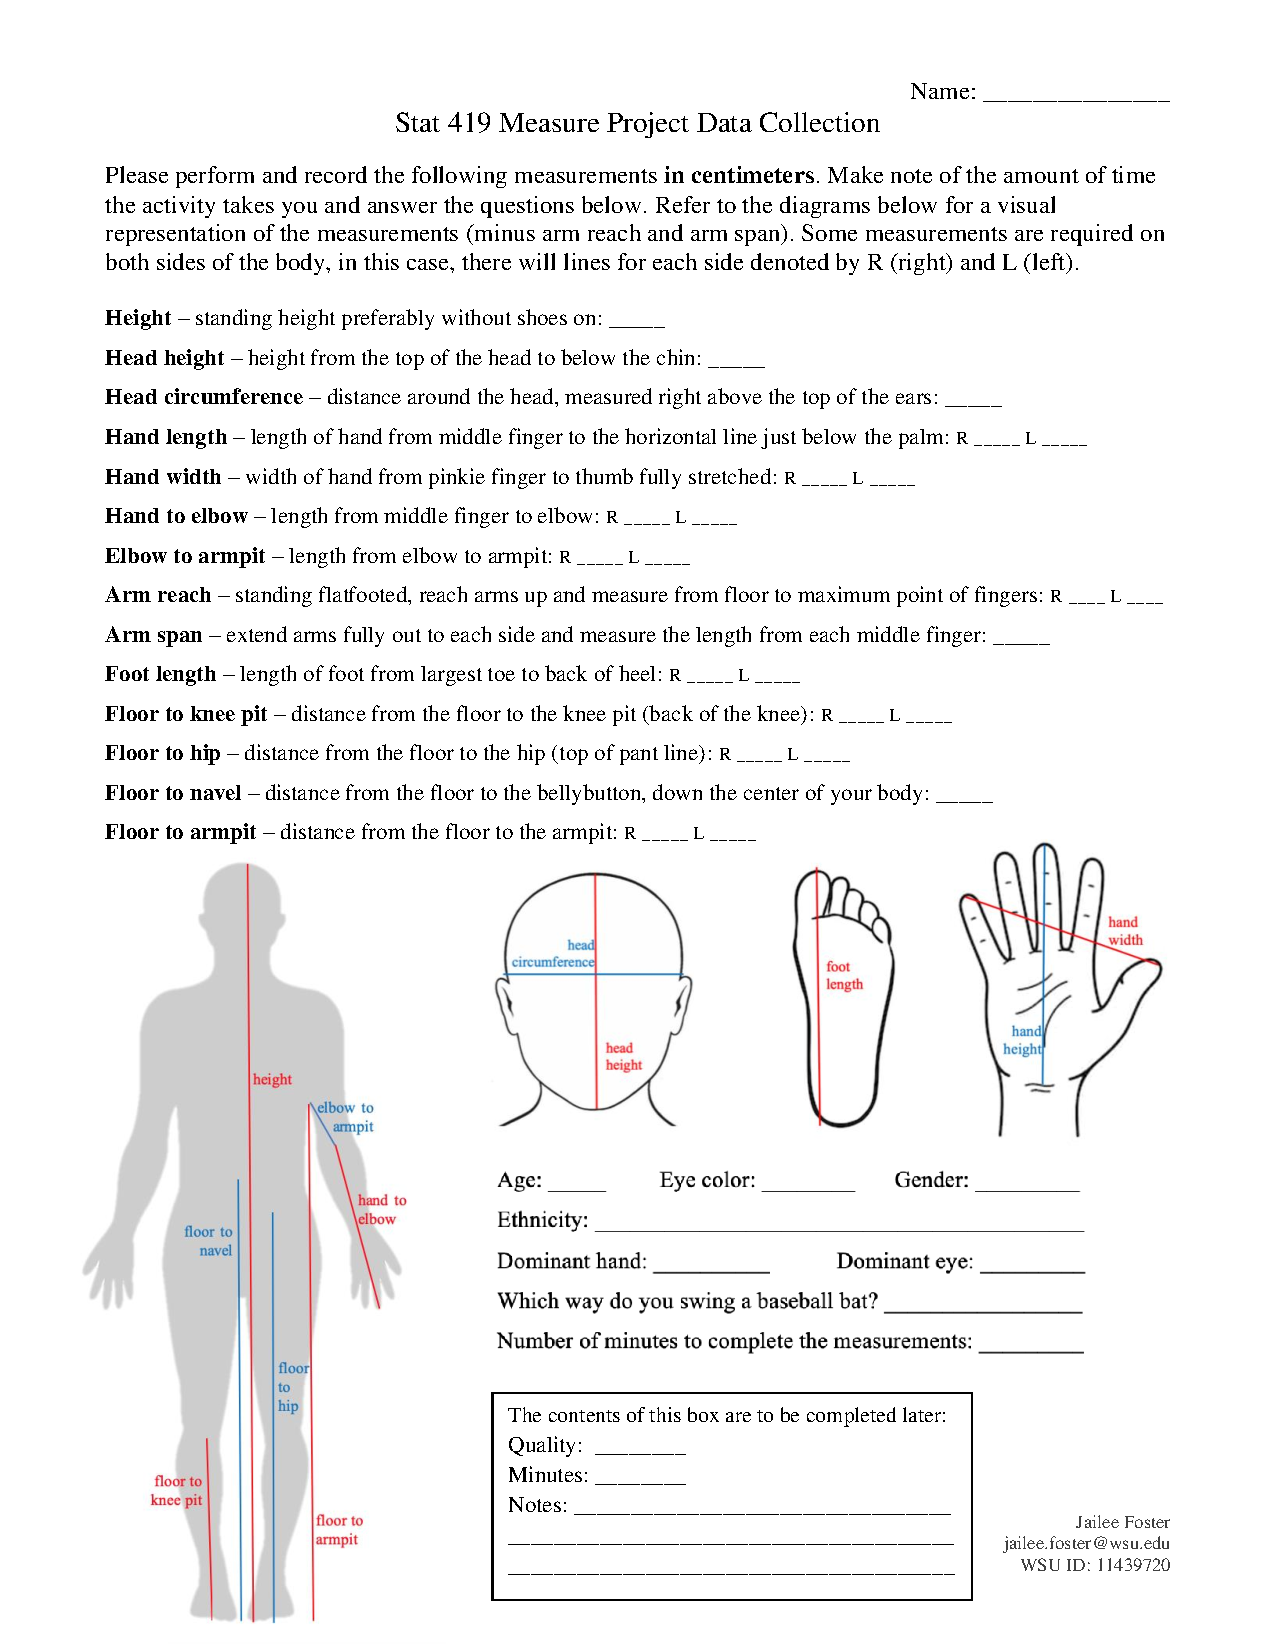
\includegraphics[trim = 0 0 0 0,clip,width=0.85\textwidth]{pdfs/handout.pdf} }
    \end{center}
    \label{fig:handout-1}
    \hrule
\end{figure}

\newpage

\subsection{Analysis}
\subsubsection{Updating Libraries and Sourcing Functions}

Below are the necessary functions and libraries required to run the code
referenced in this document.

\begin{Shaded}
\begin{Highlighting}[]
\CommentTok{\# load libraries}

\FunctionTok{library}\NormalTok{(devtools);       }\CommentTok{\# required for source\_url}
\FunctionTok{library}\NormalTok{(humanVerseWSU);  }\CommentTok{\# if humanVerseWSU is installed on machine}

\CommentTok{\# source functions }

\NormalTok{path.humanVerseWSU }\OtherTok{=} \StringTok{"https://raw.githubusercontent.com/MonteShaffer/humanVerseWSU/"}
\FunctionTok{source\_url}\NormalTok{( }\FunctionTok{paste0}\NormalTok{(path.humanVerseWSU,}\StringTok{"master/misc/functions{-}project{-}measure.R"}\NormalTok{) );}

\CommentTok{\# github.path = "https://raw.githubusercontent.com/jaileefoster/WSU\_STATS419\_FALL2020/";}
\CommentTok{\# source\_url(paste0(github.path, "master/functions/functions{-}project{-}measure.R"));}

\NormalTok{local.path }\OtherTok{=} \StringTok{"/Users/jaileefoster/Desktop/stat419/\_git\_/WSU\_STATS419\_FALL2020/"}\NormalTok{;}
\FunctionTok{source}\NormalTok{(}\FunctionTok{paste0}\NormalTok{(local.path, }\StringTok{"functions/functions{-}project{-}measure.R"}\NormalTok{), }\AttributeTok{local=}\NormalTok{T)}
\end{Highlighting}
\end{Shaded}

\subsubsection{Prepare the Data for Analysis}

Below is the code to load the data into a data frame and prepare it for
analysis. This process included determining specific columns to be used
in analysis, discarding any NA values, and checking for and removing any
extreme outliers. At this time, three new columns were added to the data
frame, one of which represented height as a factor of the person's foot
length, one representing height as a factor of the person's hand length,
and the last representing height as a factor of the person's head
height.

\begin{Shaded}
\begin{Highlighting}[]
\CommentTok{\# load the data}

\NormalTok{path.to.secret }\OtherTok{=} \StringTok{"/Users/jaileefoster/Desktop/stat419/\_git\_/secret/"}\NormalTok{;}
\NormalTok{measure.df }\OtherTok{=} \FunctionTok{read.csv}\NormalTok{( }\FunctionTok{paste0}\NormalTok{(path.to.secret, }\StringTok{"final.measure.txt"}\NormalTok{), }\AttributeTok{header=}\ConstantTok{TRUE}\NormalTok{, }
                           \AttributeTok{quote=}\StringTok{""}\NormalTok{, }\AttributeTok{sep=}\StringTok{"|"}\NormalTok{);}

\CommentTok{\# save the prepared data in a new data frame}

\NormalTok{measure.clean }\OtherTok{=} \FunctionTok{prepareMeasureData}\NormalTok{(measure.df);}
\end{Highlighting}
\end{Shaded}

\subsubsection{Generate Correlation Table}

Below is the code to generate the summary statistics, mean and standard
deviation, and correlation coefficients and save them in the table that
you see in Section \ref{sec:data-summary}.

\begin{Shaded}
\begin{Highlighting}[]
\CommentTok{\# set table directory}

\NormalTok{path.tables }\OtherTok{=} \StringTok{\textquotesingle{}/Users/jaileefoster/Desktop/stat419/\_git\_/WSU\_STATS419\_FALL2020/project{-}measure/tables/\textquotesingle{}}
\FunctionTok{createDirRecursive}\NormalTok{(path.tables)}

\CommentTok{\# create correlation table}

\NormalTok{file.correlation }\OtherTok{=} \FunctionTok{paste0}\NormalTok{(path.tables,}\StringTok{"measure{-}table{-}final.tex"}\NormalTok{) }
\NormalTok{myData }\OtherTok{=} \FunctionTok{as.matrix}\NormalTok{(measure.clean)}

\FunctionTok{buildLatexCorrelationTable}\NormalTok{(myData, }
                           \AttributeTok{rotateTable =} \ConstantTok{TRUE}\NormalTok{, }
                           \AttributeTok{width.table =} \FloatTok{0.9}\NormalTok{, }
                           \AttributeTok{myFile =}\NormalTok{ file.correlation, }
                           \AttributeTok{showOnes =} \StringTok{"center"}\NormalTok{,}
                           \AttributeTok{width.names =} \StringTok{"50mm"}\NormalTok{,}
                           \AttributeTok{myNames =} \FunctionTok{c}\NormalTok{(}\StringTok{"Height (in)"}\NormalTok{, }\StringTok{"Foot Length (in)"}\NormalTok{, }
                                       \StringTok{"Hand Length (in)"}\NormalTok{, }\StringTok{"Head Height (in)"}\NormalTok{, }
                                       \StringTok{"Height (in foot lengths)"}\NormalTok{, }
                                       \StringTok{"Height (in hand lengths)"}\NormalTok{, }
                                       \StringTok{"Height (in head heights)"}\NormalTok{), }
                           \AttributeTok{myCaption =} \StringTok{"Descriptive Statistics and Correlation Analysis }
\StringTok{                                        for Measurments in Adults"}\NormalTok{)}
\end{Highlighting}
\end{Shaded}

\subsubsection{Perform T-Tests}

Below is the code used to perform the three t-tests on the three
different hypothesis. For each t-test, the null hypothesis is that the
true mean of the population of present day adults is equal to the target
obtained from the Vitruvian Man model. The alternative hypothesis for
each is that the true mean of the population of present day adults
varies from the target obtained from the Vitruvian Man model (two-sided
test). The confidence level for each of the three t-tests is 95\%
(\(\alpha = 0.05\)).

\begin{Shaded}
\begin{Highlighting}[]
\FunctionTok{performTTestOnHeightAsFactorOfFootLength}\NormalTok{(measure.clean)}
\FunctionTok{performTTestOnHeightAsFactorOfHandLength}\NormalTok{(measure.clean)}
\FunctionTok{performTTestOnHeightAsFactorOfHeadHeight}\NormalTok{(measure.clean)}
\end{Highlighting}
\end{Shaded}





%% appendices go here!


\newpage
\theendnotes

%%%%%%%%%%%%%%%%%%%%%%%%%%%%%%%%%%%  biblio %%%%%%%%
\newpage
\begin{auxmulticols}{1}
\singlespacing 
\bibliography{./../biblio/master.bib}

%%%%%%%%%%%%%%%%%%%%%%%%%%%%%%%%%%%  biblio %%%%%%%%
\end{auxmulticols}

\newpage
{
\hypersetup{linkcolor=black}
\setcounter{tocdepth}{3}
\tableofcontents
}



\end{document}